% !TEX root = ../main.tex

%************************************************
\chapter{Narrow line region properties}
\label{ch:nlr} 
%************************************************

\section{Introduction}

X-ray and \ac{UV} spectroscopy reveal high velocity outflows to be nearly ubiquitous on sub-parsec scales in high accretion rate \ac{AGN}.
Models of galaxy evolution that invoke \ac{AGN} feedback require these outflows to reach galactic scales and quench star formation in the \ac{AGN} host galaxy. 
In recent years, a huge amount of resources have been devoted to searching for observational evidence of galaxy-wide, \ac{AGN}-driven outflows. 
This has resulted in recent detections of winds in \ac{AGN}-host galaxies using tracers of atomic, molecular, and ionised gas \citep[e.g.][]{nesvadba06,arav08,nesvadba08,moe09,dunn10,alexander10,harrison12,harrison14,nesvadba10,rupke13,veilleux13,nardini15,feruglio10,alatalo11,cimatti13,cicone14}.  

One particularly successful technique has been observing forbidden emission lines, which trace warm (T$\sim$$10^4$K) ionised gas in the \ac{NLR}. 
Because of its high equivalent width, [\ion{O}{III}]\l5008 is the most studied of the narrow \ac{AGN} emission lines. 
In general, the [\ion{O}{III}] emission consists of two components: a narrow, `core' component, with a velocity close to the systemic redshift of the host galaxy, and a broader `wing' component, which is normally blueshifted. 
The general consensus is that the core component traces the gravitational potential of the host galaxy, as the width correlates well with the stellar velocity dispersion. 
On the other hand, the broad, blueshifted wing is tracing outflowing gas. 
This emission appears blueshifted because the far-side of the outflow - that is, the side which is moving away from the line of sight - is obscured \citep[e.g.][]{heckman81,vrtilek85}. 

Observations of broad velocity-widths and blueshifts in narrow emission lines stretch back several decades \citep[e.g.][]{weedman70,stockton76,heckman81,veron81,feldman82,heckman84,vrtilek85,whittle85,boroson92}. 
However, these studies rely on small samples, which are often unrepresentative of the properties of the population. 
More recently, the advent of large optical spectroscopic surveys (e.g. \ac{SDSS}) have facilitated studies of the \ac{NLR} in tens of thousands of \ac{AGN} \citep[e.g.][]{boroson05,greene05a,zhang11,mullaney13,zakamska14,shen14}. 
This has provided constraints on the prevalence and drivers of ionised outflows.   
At the same time, there is strong evidence from spatially resolved spectroscopic observations that these outflows are extended over galaxy scales \citep[e.g.][]{greene09,greene11,hainline13,harrison12,harrison14}. 

However, these studies do not cover the redshift range when star formation and \ac{BH} accretion peaked, and consequently when feedback is predicted to be strongest. 
At these redshifts the bright optical emission lines are redshifted to near-infrared wavelengths, where observations are much more challenging. 
As a consequence, studies at high redshifts have typically relied on relatively small numbers of objects \citep[e.g.][]{netzer04,sulentic04,shen16a}.
These studies find [\ion{O}{III}] to be broader in more luminous \ac{AGN}, suggesting that \ac{AGN} efficiency in driving galaxy-wide outflows increases with luminosity \citep[e.g.][]{netzer04,nesvadba08,kim13,brusa15,carniani15,perna15,bischetti16}. 
In addition, [\ion{O}{III}] is often very weak, or is missing entirely in luminous \ac{AGN} \citep[e.g.][]{netzer04}. 

Other recent studies have looked at the [\ion{O}{III}] emission properties of extreme objects - e.g. heavily obscured quasars \citep{zakamska16} and the most luminous quasars \citep{bischetti16} - at redshifts $z\sim2$. 
The [\ion{O}{III}] emission in these objects is very broad and strongly blueshifted. 
These observations are consistent with galaxy formation models that predict \ac{AGN} feedback to be strongest in luminous, dust-obscured quasars.

In this chapter we analyse the [\ion{O}{III}] properties of a sample of 356 high-luminosity, redshift $1.5 < z < 4$ quasars.
This is the largest study of the narrow line region properties of high redshift quasars ever undertaken. 
The large sample size will help to put observations of extreme objects in context of the \ac{AGN} population as a whole.
We will analyse the [\ion{O}{III}] emission properties as a function of key properties of the quasar, e.g. \ac{BH} mass, luminosity, and accretion rate. 

\section{Quasar Sample}

From our \ac{NIR} spectroscopic catalogue (Chapter~\ref{ch:nirsample}), we have selected 356 quasars which have spectra covering the strong, narrow [\ion{O}{III}] doublet. 
The broad Balmer \hb line is also observed for all but two of the sample. 
In 165 the spectra extend to the broad \ha emission at 6565\AA, and in 260 optical spectra including \ion{C}{IV} are also available (mostly from \ac{SDSS}/\ac{BOSS}). 
The sample, which has a redshift range $1.5 < z < 4$, is summarised in Table~\ref{tab:specnums_ch4}.

\begin{table}
  \centering
  \small 
  \caption{The numbers of quasars with [\ion{O}{III}] line measurements and the spectrographs and telescopes used to obtain the near-infrared spectra.}
  \label{tab:specnums_ch4}
    \begin{tabular}{ccc} 
    \hline
    Spectrograph & Telescope & Number \\
                 &           & \\
    \hline
    FIRE         & MAGELLAN  & 31 \\
    GNIRS        & GEMINI-N  & 28 \\
    ISAAC        & VLT       & 9 \\
    LIRIS        & WHT       & 7 \\
    NIRI         & GEMINI-N  & 29 \\
    NIRSPEC      & Keck II   & 3 \\
    SINFONI      & VLT       & 80 \\
    SOFI         & NTT       & 76 \\
    TRIPLESPEC   & ARC-3.5m  & 27 \\
    TRIPLESPEC   & P200      & 45 \\
    XSHOOTER     & VLT       & 21 \\
    \hline
    \multicolumn{2}{c}{Total} & 356 \\
    \hline
    \end{tabular}
\end{table} 

\section{Parametric Model Fits}

In this section we describe how parameters of the [\ion{O}{III}] emission are derived. 
Our approach is to model the spectra using a power-law continuum, an empirical \ion{Fe}{II} template and multiple Gaussian components to model the emission from the broad and narrow components of \hb and the [\ion{O}{III}] doublet.
This is a model which is commonly adopted in the literature \citep[e.g.][]{shen11}. 
We then derive emission line parameters from the best-fitting models. 
The model-fitting is procedure is more robust when analysing spectra with limited \ac{S/N} (in comparison to measuring line properties directly from the data) and allows the emission from different transitions to be isolated. 

\subsection{Description of model}

Before a spectrum can be modelled, it must first be transformed to the quasar rest-frame.  
The redshift used in this transformation is either derived from the peak of the broad \ha emission ($\sim$ 40 per cent of our sample), from the peak of the broad \hb emission ($\sim$ 40 per cent) or from the peak of the narrow [\ion{O}{III}] emission (20 per cent).
The rest-frame transformation is only required to be accurate to within $\sim$1000\kms\, for our fitting procedure to work. 
In later sections, more precise estimates of the systemic redshift will be calculated using our parametric model fits to the [\ion{O}{III}] emission. 

The continuum and \ion{Fe}{II} emission is first modelled and subtracted using the procedure described in Chapter~\ref{ch:bhmass}. 
The \hb and [\ion{O}{III}] emission is then fit, again using the procedure described in Chapter~\ref{ch:bhmass}. 
However, we make a number of modifications to the parametric model employed in the fit, which we now describe. 

In general, \hb is modelled by two Gaussians with non-negative amplitudes and \ac{FWHM} greater than 1200\kms.
In 10 objects \hb is modelled with a single Gaussian and in 41 objects \hb is modelled with two Gaussians, but the velocity centroids of the two Gaussians are constrained to be equal. 
These spectra generally have low \ac{S/N}, and adding extra freedom to the model does not significantly decrease the minimised reduced $\chi^2$.
In addition there are cases where the blue wing of the \hb emission is below the lower wavelength limit of the spectrograph; in these cases models with more freedom are insufficiently constrained by the data.    

Contributions to the \hb emission from the narrow-line region is weak in the vast majority of our sample, and in general we do not include an additional Gaussian component to model this emission. 
In 9 objects features in the model - data residuals suggest that a narrow emission component is significant, and an additional narrow Gaussian is included for these quasars. 
It is likely that there is some not insignificant contribution from the narrow line region in other quasars in our sample. 
If this is the case then measures of the \hb velocity width will be biased to lower values on average. 
However, measurements of the [\ion{O}{III}] emission (the focus of this chapter) will not be affected by not decomposing \hb in separate broad and narrow components.  

Each component of the [\ion{O}{III}] doublet is fit with one or two Gaussians, depending on the fractional reduced $\chi^2$ difference between the one- and two-component models. 
Concretely, if the addition of the second Gaussian decreases the reduced $\chi^2$ by more than 5 per cent then the double-Gaussian model is accepted.
One hundred and thirty-one are fit with a single Gaussian and 154 with two Gaussians. 
When a single Gaussian is used to model each line, the peak flux ratio of the [\ion{O}{III}] 4960\,\AA\, and 5008\AA\, components are fixed at the expected 1:3 ratio and the width and velocity offsets are set to be equal.
In the double Gaussian model, the peak flux ratio of the additional components is again fixed at 1:3, and the width and velocity offsets are again set to be equal. 

In 71 objects [\ion{O}{III}] is undetected, or is detected with very low \ac{S/N}. 
In these cases we do not attempt to measure the width of the [\ion{O}{III}] emission, but determine only the normalisation of a fixed [\ion{O}{III}] template.
To generate this template we generate a median composite spectrum from the continuum- and \ion{Fe}{II}-subtracted spectra of the XX quasars with reliable [\ion{O}{III}] line measurements (see below). 
We then run our line-fitting routine on the composite spectrum, and use the best-fitting [\ion{O}{III}] model as a template. 

Some example fits are shown in Figure~\ref{fig:example_spectrum_grid}

\begin{figure}
    \centering
    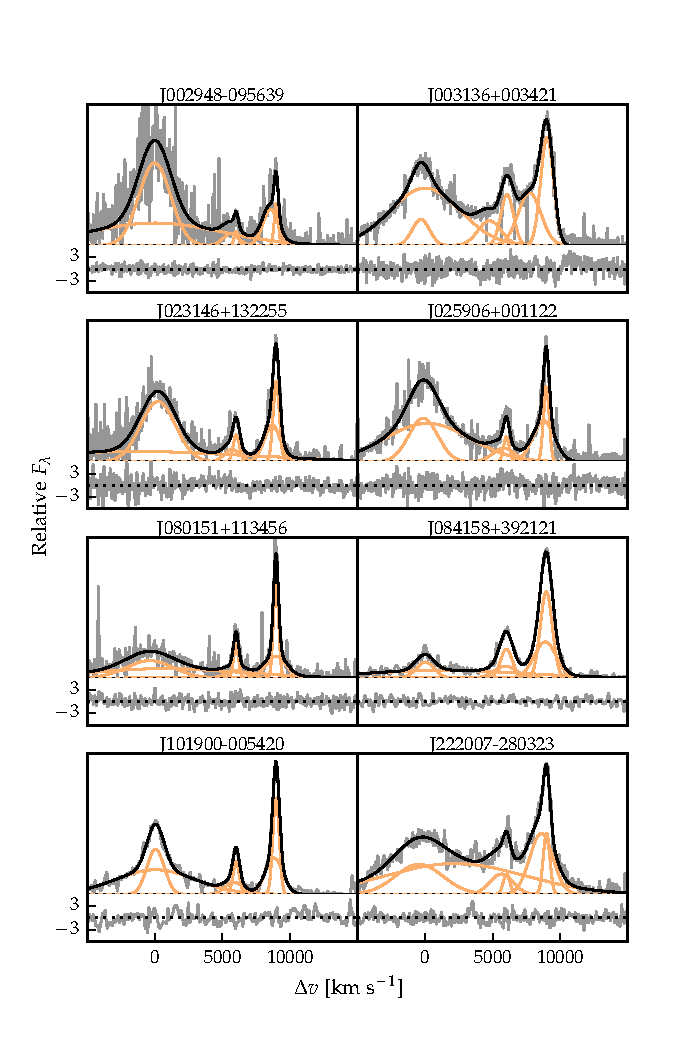
\includegraphics[width=\textwidth]{figures/chapter04/example_spectrum_grid.pdf} 
    \caption{Model fits to the continuum- and \ion{Fe}{II}-subtracted \hbns/[\ion{O}{III}] emission in 15 quasars, chosen at random. The data is shown in grey, the best-fitting model in black, and the individual model components in orange. The peak of the [\ion{O}{III}] emission is used to set the redshift, and $\Delta{v}$ is the velocity shift from the rest-frame transition wavelength of \hb. Below each spectrum we plot the data minus model residuals, scaled by the errors on the fluxes.}     
    \label{fig:example_spectrum_grid}
\end{figure}

\subsection{Derived parameters}

All [\ion{O}{III}] line properties are derived from the [\ion{O}{III}]\l5008 emission, but, as described above, the kinematics of [\ion{O}{III}]\l4960 are constrained by our fitting routine to be identical.

We do not attach any physical meaning to the individual Gaussian components used in the model. 
Decomposing the [\ion{O}{III}] emission in to a narrow component component at the systemic redshift and a lower-amplitude, blueshifted broad component is subject to large uncertainties and is highly dependent on the spectral \ac{S/N} and resolution. 
Furthermore, there is no theoretical justification that the broad component should have a Gaussian profile.  

We therefore choose to characterize the [\ion{O}{III}] line profile using a number of non-parametric measures, which are commonly used in the literature \citep[e.g.][]{zakamska14,zakamska16}. 
A normalised cumulative velocity distribution is constructed from the best-fitting model, from which the velocities below which 5, 10, 25, 50, 75, 90, and 95 per cent of the total flux accumulates can be calculated. 
The width of the emission line can then be defined, for example, using $w_{80} \equiv v_{90} - v_{10}$. 
We also define the absolute asymmetry in the line profile $A$ as $((v_{95} - v_{50}) - (v_{50} - v_{5})) / (v_{95} - v_{5})$ \citep[e.g.][]{zakamska14}. 
\todo{The line width measures are not corrected for instrumental broadening}
\todo{Add outline of table of derived properties for this chapter}

\subsection{Flux calibration of spectra}

We established the absolute flux scale for each near-infrared spectrum using a similar methodology to the one described in Chapter~\ref{ch:bhmass}. 
If near-infrared photometric data was available for our whole sample then this could be used to establish the absolute flux scale of the near-infrared spectra. 
Because this information is missing for a sizeable fraction of our sample, we instead consider two approaches. 

In the first approach, we leverage the excellent flux-calibration of the \ac{SDSS}/\ac{BOSS} spectra, which are available for XX objects in our sample. 
We use our standard quasar \ac{SED} model (Chapter~\ref{ch:sed}) to bridge the gap between the wavelength coverage of the near-infrared and optical \ac{SDSS}/\ac{BOSS} spectra.
The quasar \ac{SED} model is fit to the \ac{SDSS}/\ac{BOSS} spectra, with the normalisation and extinction E(B-V) as free parameters. 
The near-infrared spectra are then normalised to the \ac{SED} model using a linear error weighted least-squares regression.  
The second approach is identical, except rather than using the \ac{SDSS}/\ac{BOSS} spectra we fit the same \ac{SED} model to the available photometric data from the optical (\ac{SDSS}) to the near-infrared (VHS, Viking, UKIDSS, 2MASS). 

The monochromatic continuum luminosity - used as a proxy for the \ac{AGN} bolometric luminosity - is also used below. 
This is calculated in the same way as in Chapter~\ref{ch:bhmass}. 
\todo{Check if any missing normalisation / monochromatic luminosities.} 
\todo{Check factor of (1+z) in luminosity calculation}


% The reported line-width measures are corrected for instrumental broadening by subtracting the resolution of the spectrograph in quadrature. 
% The spectrograph resolutions, which we estimate from the line widths in the observed sky spectra, are given in Table XX. 

% \begin{table}
%   \centering
%   \small 
%   \caption{Measured spectral resolutions of the spectrographs used in this thesis.}
%   \label{tab:specnums_ch4}
%     \begin{tabular}{ccc} 
%     \hline
%     Spectrograph & Telescope & Number \\
%                  &           & \\
%     \hline
%     FIRE         & MAGELLAN  & 31 \\
%     GNIRS        & GEMINI-N  & 28 \\
%     ISAAC        & VLT       & 9 \\
%     LIRIS        & WHT       & 7 \\
%     NIRI         & GEMINI-N  & 29 \\
%     NIRSPEC      & Keck II   & 3 \\
%     SINFONI      & VLT       & 80 \\
%     SOFI         & NTT       & 76 \\
%     TRIPLESPEC   & ARC-3.5m  & 27 \\
%     TRIPLESPEC   & P200      & 45 \\
%     XSHOOTER     & VLT       & 21 \\
%     \hline
%     \multicolumn{2}{c}{Total} & 356 \\
%     \hline
%     \end{tabular}
% \end{table} 



%     # instr_width = {'GNIRS':136.0, 
%     #                'NIRSPEC':122.0, 
%     #                'XSHOOT':25.0, 
%     #                'NIRI':465.0, 
%     #                'ISAAC':46.0, 
%     #                'TRIPLE_P200':88.0, 
%     #                'SOFI_MR':323.0, 
%     #                'LIRIS':477.0, 
%     #                'SOFI_LR':535.0,
%     #                'FIRE':59.0,
%     #                'TRIPLE_ARC':97.0,
%     #                'SINF':124.0}




\subsection{Reliability of derived parameters}

\subsubsection{Removal of \ion{Fe}{II} emission}

\begin{figure}
    \centering
    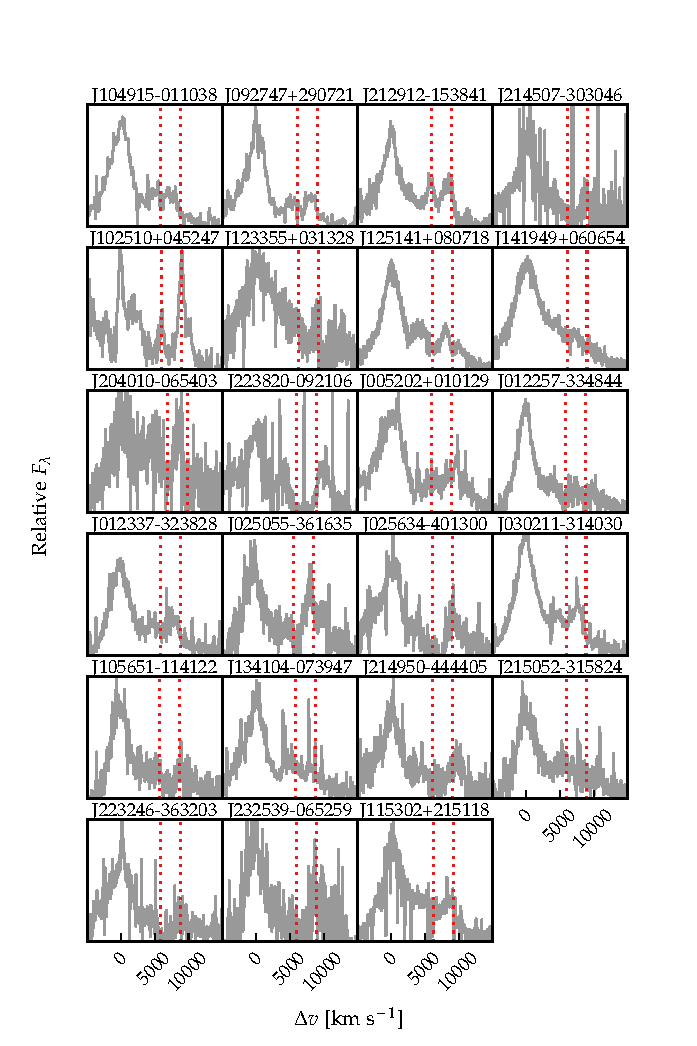
\includegraphics[width=\columnwidth]{figures/chapter04/example_spectrum_grid_extreme_fe.pdf} 
    \caption{Spectra of the 23 objects for which significant \ion{Fe}{II} emission is still visible following our \ion{Fe}{II}-subtraction procedure. The vertical lines indicate the expected positions of the [\ion{O}{III}] doublet (which is generally very weak) with the systemic redshift defined using the peak of the broad \hb emission.}     
    \label{fig:bad_fe}
\end{figure}

We encountered 23 cases where the relative strengths of the \ion{Fe}{II} lines appear to differ significantly from those of I Zw 1 on which the \ion{Fe}{II} template we use is based. 
As a result, significant \ion{Fe}{II} flux remained in the spectra after the removal process. 
This emission is at rest-frame wavelengths very close to the [\ion{O}{III}] emission, and so could potentially lead to large errors in the inferred [\ion{O}{III}] line parameters. 
In Figure~\ref{fig:bad_fe} we plot the spectral region around [\ion{O}{III}] these 23 objects.
The vertical lines indicate the expected positions of the [\ion{O}{III}] doublet, with zero velocity defined using the peak of the broad \hb emission. 
[\ion{O}{III}] is generally extremely weak in these objects. 
As a result, fitting multiple Gaussians will tend to fit the \ion{Fe}{II} emission as broad, shifted [\ion{O}{III}]. 
For example, J125141+080718 was studied by \citet{shen16a}, and assigned an extremely large [\ion{O}{III}] blueshift. 
Our analysis suggests that this emission is more likely to be \ion{Fe}{II}. 
Because of the difficulty measuring the [\ion{O}{III}] properties of these objects, they are excluded from subsequent analysis.  

\subsubsection{Low \ac{EQW} [\ion{O}{III}]}

\begin{figure}
    \centering
    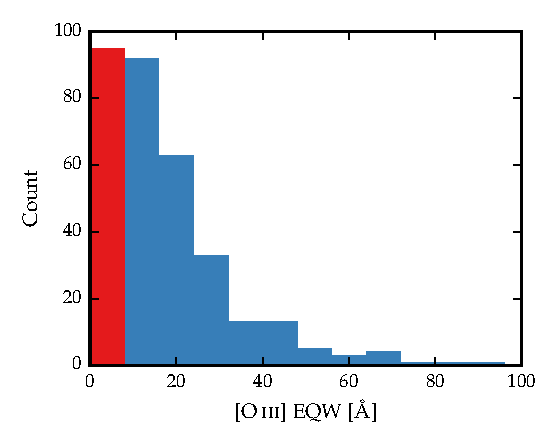
\includegraphics[width=0.7\textwidth]{figures/chapter04/oiii_eqw_hist.pdf} 
    \caption{[\ion{O}{III}] \ac{EQW}. The [\ion{O}{III}] profiles of the 120 objects in the red bin (\ac{EQW} $<$ 8\AA) cannot be measured reliably using our model-fitting procedure.}     
    \label{fig:oiii_strength_hist}
\end{figure}

In Figure~\ref{fig:oiii_strength_hist} we show the distribution of the [\ion{O}{III}] rest-frame \ac{EQW} distribution for the 330 objects in our sample (objects where \ion{Fe}{II} emission has been sub-optimally removed are excluded). 
In many objects [\ion{O}{III}] is undetected. 
In others it is detected, but is too weak for its shape (i.e. the width and asymmetry) to be measured reliably. 
We define \ac{EQW}$=8$\AA\, as the limit below which we can no longer reliably determine the shape of the [\ion{O}{III}] emission. 
Objects with \ac{EQW}$<8$\AA\, (120) are excluded in subsequent analysis of the [\ion{O}{III}] shape.  
\todo{Can I justify quantitatively why this limit is chosen?}

\subsubsection{Low \ac{S/N} [\ion{O}{III}]}
 
\begin{figure}
    \centering
    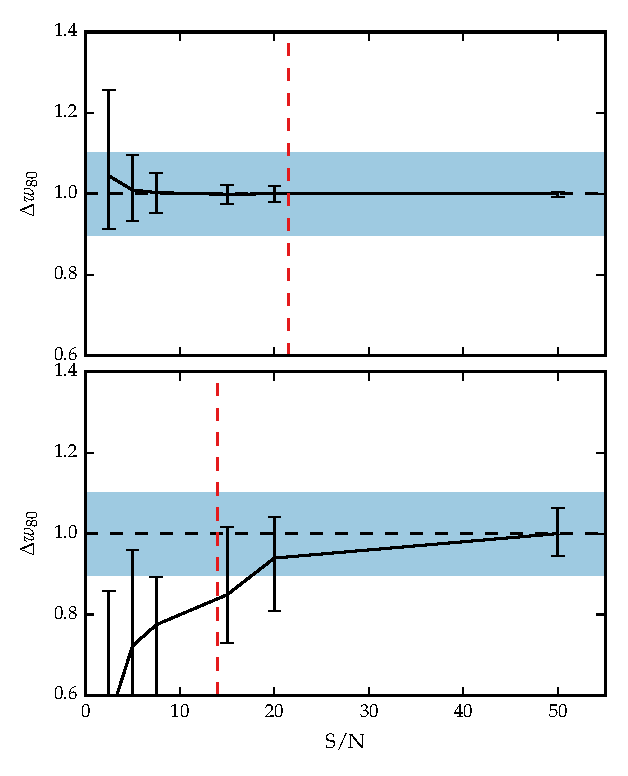
\includegraphics[width=0.7\columnwidth]{figures/chapter04/snr_test.pdf} 
    \caption{Fractional change in the [\ion{O}{III}] line parameter $w_{80}$ as a function of the \ac{S/N} of six simulated spectra. At each \ac{S/N}, our line-fitting procedure is run on 100 mock spectra, and the points and error-bars indicate the 50th percentile and 16-84 percentile range respectively. The $w_{80}$ parameter is considered `unreliable' if $|\Delta w_{80}|>0.1$ at the \ac{S/N} of the real spectrum (represented by the vertical line). Our $w_{80}$ measurement is `reliable' for J100627+480420 and `unreliable' for J124948+060714.}
    \label{fig:snr_test}
\end{figure}

In this section we flag objects with poor spectral \ac{S/N}. 
A single \ac{S/N} cut is not adequate because, for a given \ac{S/N}, it is much easier to measure the properties of a strong line than a weaker one. 
Our approach is therefore as follows:

\begin{enumerate}
\item For each object, we use the best-fitting parametric model as a high \ac{S/N} representation of the spectra. 
\item We scale the error spectrum so that the \ac{S/N} (measured in the continuum and quoted per pixel) is \{2.5, 5, 7.5, 10, 15, 20, 50\}.
\item At each \ac{S/N}, we generate 100 mock spectra by randomly drawing the flux in each pixel from a Normal distribution with mean $\mu$ equal to the model flux and width $\sigma$ equal to the scaled error. 
\item We run our line-fitting procedure on each of the 100 mock spectra and record the value of $w_{80}$ in the best-fitting model. 
\item We calculate the 16th, 50th and 84th percentiles of the distribution of $w_{80}$ values.
\item We calculate the the median $w_{80}$ value at \ac{S/N}$=50$ and at the \ac{S/N} of the real spectrum (by linearly interpolating between the results of our simulations). The low \ac{S/N} flag is assigned to the object if the median $w_{80}$ changes by more than 10 per cent between these two \ac{S/N} realisations. 
\end{enumerate}

Examples of this test for two different objects are shown in Figure~\ref{fig:snr_test}.
The marker denotes the 50th percentile, and the lower and upper error bars the 16th and 84th percentiles respectively. 
As expected, the uncertainty on $w_{80}$ increases as the \ac{S/N} of the spectrum decreases. 
The \ac{S/N} in to two spectra are similar, but the [\ion{O}{III}] line in the  first object is stronger. 
Hence it can still be measured reliably even at low \ac{S/N}. 
The first object would passes our \ac{S/N} cut, whereas the latter fails it. 

\todo{Need some discussion on how much v95 and v05 in particular depend on SNR. You have some discussion about making sure w80 is robust to SNR changes. Did you also do similar tests for v95, v05, v10 etc?}

\section{Reliability of redshift estimates}

\begin{figure}
    \centering
    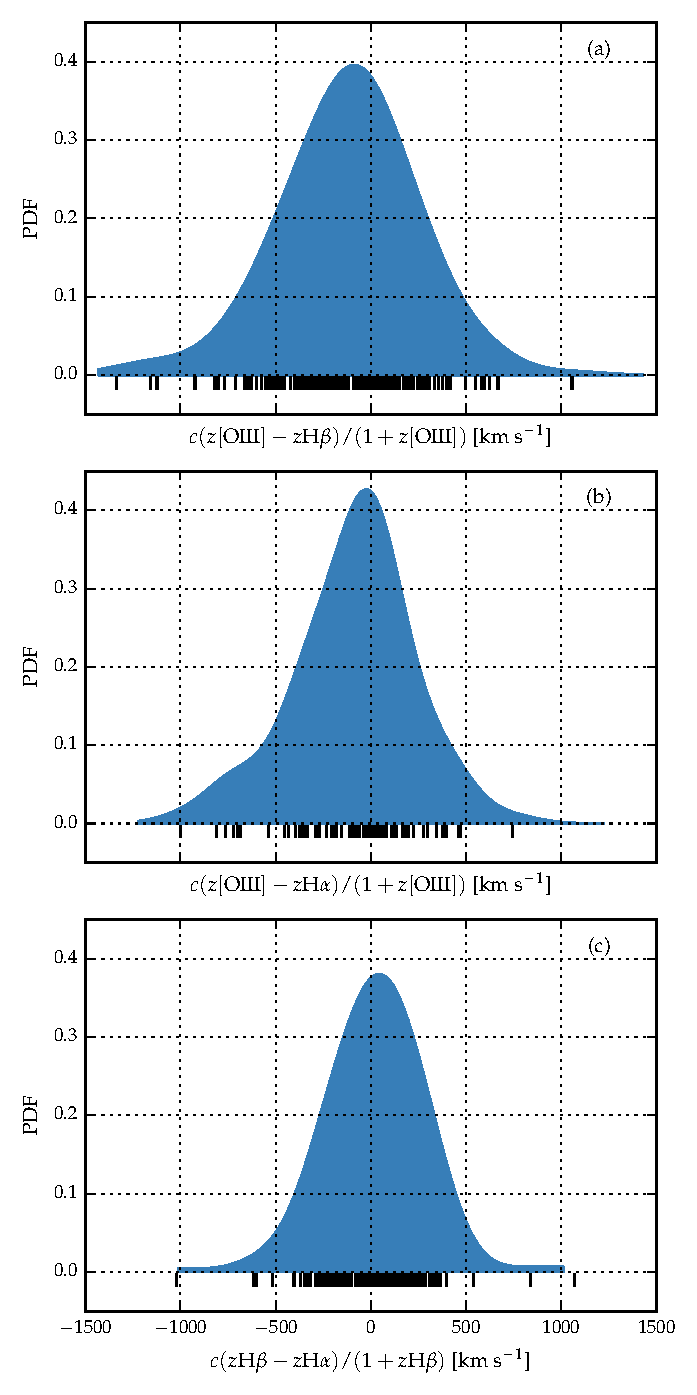
\includegraphics[width=0.8\linewidth]{figures/chapter04/redshift_comparison.pdf} 
    \caption{Comparison of systemic redshift estimates using [\ion{O}{III}], broad \hb and broad \hans. In all cases the line location is defined as the peak wavelength of the best-fitting model. There are 93, 73 and 83 objects in (a), (b) and (c) respectively. The mean and standard deviation have been calculated by fitting a Gaussian function (shown in red) to the distribution. \todoinline{Need to look at flags>1 for \ha and \hb.} \todoinline{Is peak around zero in (a) real?} \todoinline{Is it clear in text which quasars are going in to each subfigure?}}       
    \label{fig:redshift_comparison}
\end{figure}

In this section we do a comparison of systemic redshift estimates from [\ion{O}{III}], broad \hb and \hans. 
This is an important issue. 
Accurate systemic redshift estimates are essential in a number of applications, and researchers have devoted a large amount of telescope time to obtaining near-infrared spectra to access [\ion{O}{III}] for this purpose. 
HI, CO and absorption line measures of the host galaxy rest frame suggest that [\ion{O}{III}] usually gives consistent results within 200\kms (de Robertis 1985; Whittle 1985; Wilson \& Heckman 1985; Condon et al. 1985; Stripe 1990; Alloin et al. 1992; Evans et al. 2001).  
However, our work shows that at high luminosities this can result in large errors (profile can be dominated by blueshifted component, \ion{Fe}{II} emission can be improperly subtracted, or [\ion{O}{III}] might not be detected at all. 

\subsection{Modelling \hans}

There are 224 quasars in our sample with spectra covering the \ha emission line. 
We discard seven of these from our sample because of very low \ac{S/N} ($<$2.5 measured in the \ha line), leaving 217
To measure the position of the line we fit a parametric model, which is very similar to the model described in Chapter~\ref{ch:bhmass}. 
The continuum emission is first modeled and subtracted using the procedure described in Chapter~\ref{ch:bhmass}. 
We then test five different models with increasing degrees of freedom to model the \ha emission. 
The models are summarised in Table~\ref{tab:hamod}. 
They are (1) a single broad Gaussian; (2) two broad Gaussians with identical velocity centroids; (3) two broad Gaussians with different velocity centroids; (4) two broad Gaussians with identical velocity centroids, and additional narrower Gaussians to model the narrow \ha emission, and the narrow components of [\ion{N}{II}]\ll6548,6584 and [\ion{S}{II}]\ll6717,6731; (5) two broad Gaussians with different velocity centroids, and additional narrower Gaussians. 
If used, the width and velocity of all narrow components are set to be equal in the fit, and the relative flux ratio of the two [\ion{N}{II}] components is fixed at the expected value of 2.96.
The model we select is the simplest model for which the fractional change in the reduced $\chi^2$ from the model with the lowest reduced $\chi^2$ is less than ten per cent. 
The redshift is then measured at the peak flux of the \ha model, including both the broad and narrow components of \ha if appropriate. 

\begin{table}
  \centering
  \small 
  \caption{Models used for \ha emission.}
  \label{tab:hamod}
    \begin{tabular}{cccc} 
    \hline
    Model     & Components & Fix centroids? & Number \\
    \hline
    1        & 1 broad Gaussian  & N/A &  10 \\
    2        & 2 broad Gaussians & Yes &  71 \\
    3        & 2 broad Gaussians & No  &  32 \\
    4        & 2 broad Gaussians + narrow Gaussians & Yes & 51 \\
    5        & 2 broad Gaussians + narrow Gaussians & No  & 53 \\
    \hline
    \end{tabular}
\end{table} 

\section{Results}


\begin{figure}
    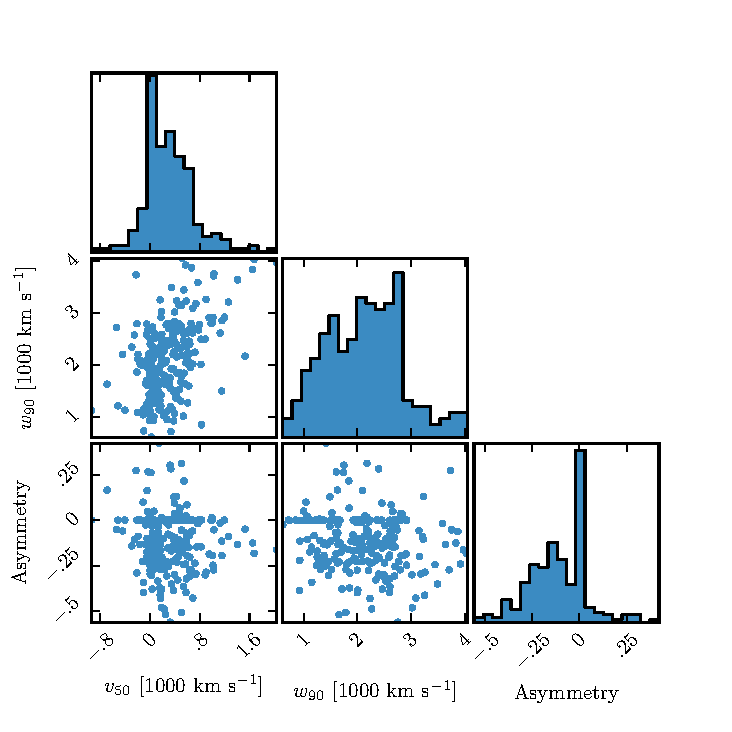
\includegraphics[width=\columnwidth]{figures/chapter04/parameters_grid.pdf} 
    \caption{Correlations between the line width $w_{80}$, asymmetry $R$ and \ac{EQW} of [\ion{O}{III}].}     
    \label{fig:parameters_grid}
\end{figure}

In our sample of XX quasars, there is a huge diversity in [\ion{O}{III}] emission properties (Fig.~\ref{fig:example_spectrum_grid}). 
In a significant fraction [\ion{O}{III}] is undetected, whereas in others the \ac{EQW} is in excess of 100\AA. 
The median is XX, which is somewhat lower than is found in lower-redshift, lower-luminosity AGN. 
$w_{80}$ varies between 400 and 3000 \kms, with a median 1500 \kms.  
When the broad wing is detected, it is almost ubiquitously blueshifted.
The luminous blueshifted broad wing and the extremely broad profile reveals high-velocity outflowing ionized gas. 
Our results therefore suggest that kilo-parsec-scale outflows in ionized gas are common in this sample of high-luminosity, high-redshift quasars.

In Figure~\ref{fig:parameters_grid} we show correlations between the [\ion{O}{III}] $w_{80}$, EQW, asymmetry for 119 quasars: objects with low \ac{EQW}, poor \ac{S/N}, poor \ion{Fe}{II} subtraction are not included. 
Objects for which [\ion{O}{III}] is modelled using a single Gaussian are also excluded, because the asymmetry is by definition zero for these objects.   
We see a correlation between the [\ion{O}{III}] velocity width and asymmetry. 
As the line gets broader it gets more blue-asymmetric. 
One interpretation of this is that the strength of the narrow core is decreasing, leading to a broader and more blueshifted profile \citep[e.g.][]{shen14}. 

\subsection{Equivalent width}

\begin{figure}
    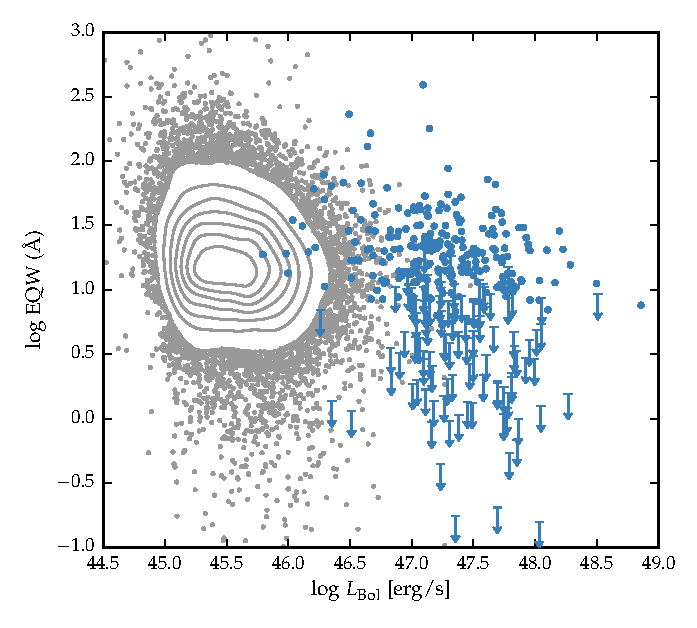
\includegraphics[width=\columnwidth]{figures/chapter04/eqw_lum.pdf} 
    \caption{The [\ion{O}{III}] \ac{EQW} as a function of the quasar bolometric luminosity for the sample presented in this chapter (blue circles) and the low-$z$ \ac{SDSS} sample (grey points and contours). Upper limits are denoted by the downward arrows.}     
    \label{fig:eqw_lum}
\end{figure}

First we discuss how upper limits on the [\ion{O}{III}] \ac{EQW} are calculated.
Firstly, the best-fitting model comprising the continuum, \ion{Fe}{II}, and \hb emission is subtracted from the spectra, leaving behind only emission due to [\ion{O}{III}]. 
From this spectra we generate 100 mock spectra, where the flux at each wavelength is randomly drawn from a Normal distribution with a mean equal to the flux convolved with a Gaussian of width 200\kms and a width equal to the known error. 
We then perform an error-weighted linear least-squares regression with an [\ion{O}{III}] template derived from a fit to a very high \ac{S/N} low redshift \ac{SDSS} composite spectra. 
The equivalent width of the best-fitting model is recorded for each of the 100 realisations of the spectra. 
The error in the equivalent width is defined as the root-mean-square of these values.

In Fig.~\ref{fig:eqw_lum} we show the [\ion{O}{III}]5008 EW as a function of the quasar bolometric luminosity. 
Bolometric luminosity is estimated from the monochromatic continuum luminosity at 5100\AA using the correction factor given by \citet{richards06}. 
For comparison, we also show the low-$z$ sample from \citet{shen11}.  

The equivalent width of [\ion{O}{III}] has been found to strongly decrease as a function of redshift and/or luminosity \citep[e.g.][]{brotherton96,netzer04,sulentic04,baskin05b}. 

The size of the narrow line region is roughly expected to scale as $L^{0.5}$ \citep[e.g.][]{netzer04}. 
However, for high luminosity quasars with strong [\ion{O}{III}] this gives \ac{NLR} sizes which are unreasonably large \citep[$\sim$100 kpc;][]{netzer04}. 

\citet{netzer04} found 1/3 of their high luminosity sample had very weak [\ion{O}{III}], whereas quasars with weak [\ion{O}{III}] are very rare for nearby \ac{AGN}. 
We find that [\ion{O}{III}] is undetected/very weak in XX per cent of our sample, which is very similar to the fraction reported by \citet{netzer04}.  
\citet{netzer04} claim that for the population of strong [\ion{O}{III}] emitters there is no reduction of EW with increasing source luminosity. 
On the other hand, there are many weak or no [\ion{O}{III}] emitters at high luminosity that could give the impression that the line \ac{EQW} decreases with increasing source luminosity. 

\todoinline{See extra text from Brotherton paper. I could be confused here, but I think the Netzer argument goes that the nlr size increase with luminosity because there are more ionising photons. but then you run out of nlr to ionise. the luminosity of the quasar keeps increasing but the luminosity of the nlr flattens out. so the eqw starts to decrease. but we see a huge scatter in eqw at high luminosities. we can relate this to the \ion{C}{IV} blueshift, which I don't think Netzer will have been able to.}


\subsubsection{Luminosity/redshift-evolution of [\ion{O}{III}] properties}

\begin{figure}
    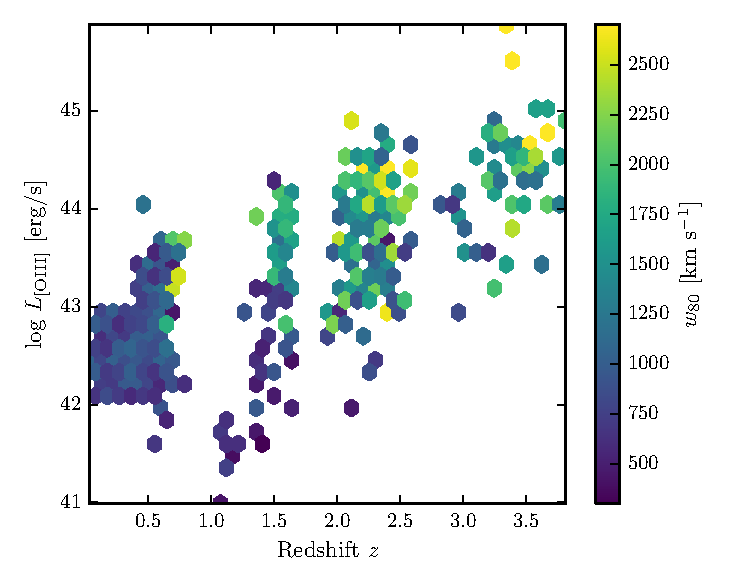
\includegraphics[width=\columnwidth]{figures/chapter04/oiii_luminosity_z_w80.pdf} 
    \caption{The [\ion{O}{III}] velocity-width, characterised by $w_{80}$, as a function the [\ion{O}{III}] luminosity and the quasar redshift. The colour of each hexagon denotes the mean $w_{80}$ for the objects in that luminosity-redshift bin. We have supplemented our sample with low-$z$ objects from \citet{zakamska14} and medium ($z\sim1.5$) redshift objects from \citet{harrison16}. \todoinline{If I keep this plot make sure its clear which points belong to which sample.}}       
    \label{fig:oiii_luminosity_z_w80}
\end{figure}

In this section we look for any luminosity/redshift dependent changes in the [\ion{O}{III}] line properties. 
To do this we extend the dynamic range of our samples in terms of both luminosity and redshift by supplementing our sample with quasars presented by \citet{zakamska14} and \citet{harrison16}. 

The \citet{zakamska14} objects are a sample of 568 obscured luminous quasars selected from \ac{SDSS} \citep{reyes08,yuan16}. 
They are selected to have [\ion{O}{III}] luminosities above $10^{8.5}{\rm L}\odot$ and have a median redshift $z=0.397$. 

We also include 40 quasars at redshifts $1.1 \leq z \leq 1.7$) from the KMOS \ac{AGN} Survey at High redshift (KASH$z$) with [\ion{O}{III}] line measurements. 

We also have the same information for $\sim$20\,000 \ac{SDSS} spectra from \citet{mullaney13}. 

In Figure~\ref{fig:oiii_luminosity_z_w80} we show the [\ion{O}{III}] velocity width as a function of the [\ion{O}{III}] luminosity and the quasar redshift. 
The [\ion{O}{III}] luminosity is calculated by 

The lack of any redshift-evolution between $z=0$ and $z=1.5$ was reported by \citet{harrison16}.
Our additional data suggests that this continues to $z\sim2.5$. 
On the other hand, at fixed redshift, we see a significant correlation between the [\ion{O}{III}] velocity width and the luminosity. 

The fact that we don't see many broad lines in the \citet{zakamska14} objects even at luminosities $>$43 erg/s could be due to the fact that these are all type II quasars, whereas the sample presented in this chapter are all type I. 
\citet{mullaney13} showed that the [\ion{O}{III}] lines of type I quasars are typically broader than in type II quasars. 

\todoinline{Need some discussion about potential selection biases in these samples e.g. Zakamska \& Green objects are obscured. Does this make a difference? Also, many studies only present detections and do not publish non-detections... I thought there were some Type 1 quasars at low-$z$ with [\ion{O}{III}] measurements from Shen? but I could be wrong.}


\subsubsection{Eigenvector 1 correlations}

\begin{figure}
    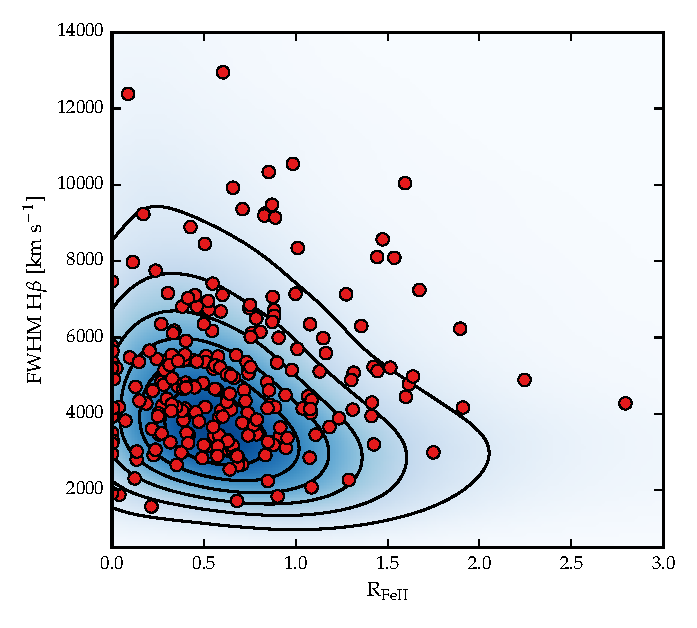
\includegraphics[width=\columnwidth]{figures/chapter04/ev1_lowz.pdf} 
    \caption{\ac{EV1} parameter space. The contours and shading show low-redshift, low-luminosity SDSS \ac{AGN} (with measurements taken from \citet{shen11}) and the red circles show the high-redshift, high-luminosity objects presented in this chapter.}      
    \label{fig:ev1_lowz}
\end{figure}

The \ac{FWHM} of the broad \hb emission line and the relative strengths of optical \ion{Fe}{II} and \hb have been identified as the features responsible for the largest variance in the spectra of AGN. 
These parameters form part of `Eigenvector 1' (EV1), the first eigenvector in a \ac{PCA} which originated from the work of \citet{boroson92}.   
The underlying driver behind EV1 is thought to be the Eddington ratio \citep[e.g.][]{sulentic00b,shen14}. 

In Figure~\ref{fig:ev1_lowz} we show the [\ion{O}{III}] \ac{EQW} as a function of the \hb \ac{FWHM} and the optical \ion{Fe}{II} strength. 
The optical \ion{Fe}{II} strength is defined as the ratio of the \ion{Fe}{II} and \hb \ac{EQW}, where the \ion{Fe}{II} \ac{EQW} is measured between 4434 and 4684\AA.
Measurements of the \hb line properties are taken from Chapter~\ref{ch:bhmass}. 
In our sample, these parameters follow very similar correlations to what is observed at low-$z$ \citep[see also][]{sulentic04, shen16a}.
In particular, the anti-correlation between the [\ion{O}{III}] and \ion{Fe}{II} \ac{EQW}.  
However, the \hb \ac{FWHM} are displaced to higher values, which is consistent with the high-redshift, high-luminosity sample having larger \ac{BH} masses. 

These emission line trends in the optical (for low-$z$ quasars) can be extended to UV emission lines observed at higher redshifts. 
The \ion{C}{IV} blueshift and \ac{EQW} is a diagnostic that similarly spans the diversity of broad emission line properties in high redshift quasars \citep[dominated by a virialized component at one extreme and a wind driven component at the other][]{richards11,sulentic07}. 
The similarity of the \ion{C}{IV} \ac{EQW}-blueshift parameter space at high redshift to \ac{EV1} parameter space at low redshift suggests that these trends are connected. 

Can we calculate a mapping between the two parameter spaces? 
As a first step we show how the \ac{EV1} parameters change as a function of position in the \ion{C}{IV} \ac{EQW}-blueshift parameter space in Figure~\ref{fig:ev1}. 
The \ion{C}{IV} blueshift is measured relative to the redshift determined from fitting the \ac{ICA} components.
Two hundred and sixty objects are shown in Figure~\ref{fig:ev1}.
Objects flagged as having significant \ion{Fe}{II} residual emission have been removed.  
Objects for which the \hb or \ion{C}{IV} line properties could not be measured reliably (see Section~\ref{sec:flagged_spectra}) have also been removed. 
Finally, we consider only objects for which the \ion{C}{IV} EQW exceeds 15\AA. 

Most of the diversity in \ion{C}{IV} properties seems to be driven by the [\ion{O}{III}] \ac{EQW}. 
On the other hand, the \ion{C}{IV} blueshift and \ac{EQW} cannot be used to predict the \hb \ac{FWHM}. 
This is consistent with what we found in Chapter~\ref{ch:bhmass}: objects with large \ion{C}{IV} blueshifts have narrow Balmer emission lines, but objects with modest \ion{C}{IV} blueshifts have a wide range of Balmer line widths. 

\begin{figure}
    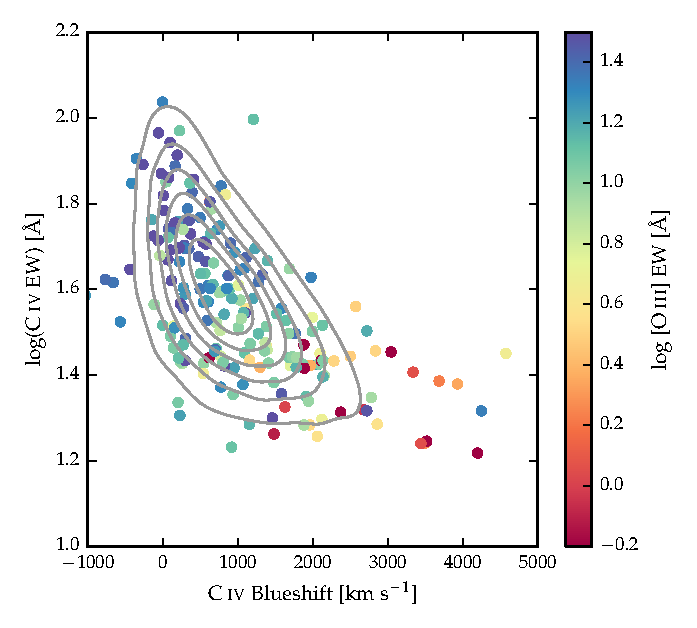
\includegraphics[width=\columnwidth]{figures/chapter04/ev1.pdf} 
    \caption{The high-redshift \ac{EV1} parameter space of \ion{C}{IV} blueshift and \ac{EQW}. Our sample is shown with points, and quasars from the full \ac{SDSS} catalogue are shown with grey contours. The [\ion{O}{III}] EQW varies systematically with position in the \ion{C}{IV} blueshift-\ac{EQW} parameter space (a) but the \hb \ac{FWHM} shows significantly less systematic variation (b).}      
    \label{fig:ev1}
\end{figure}

\subsubsection{Extreme [\ion{O}{III}]}

\begin{figure}
    \centering
    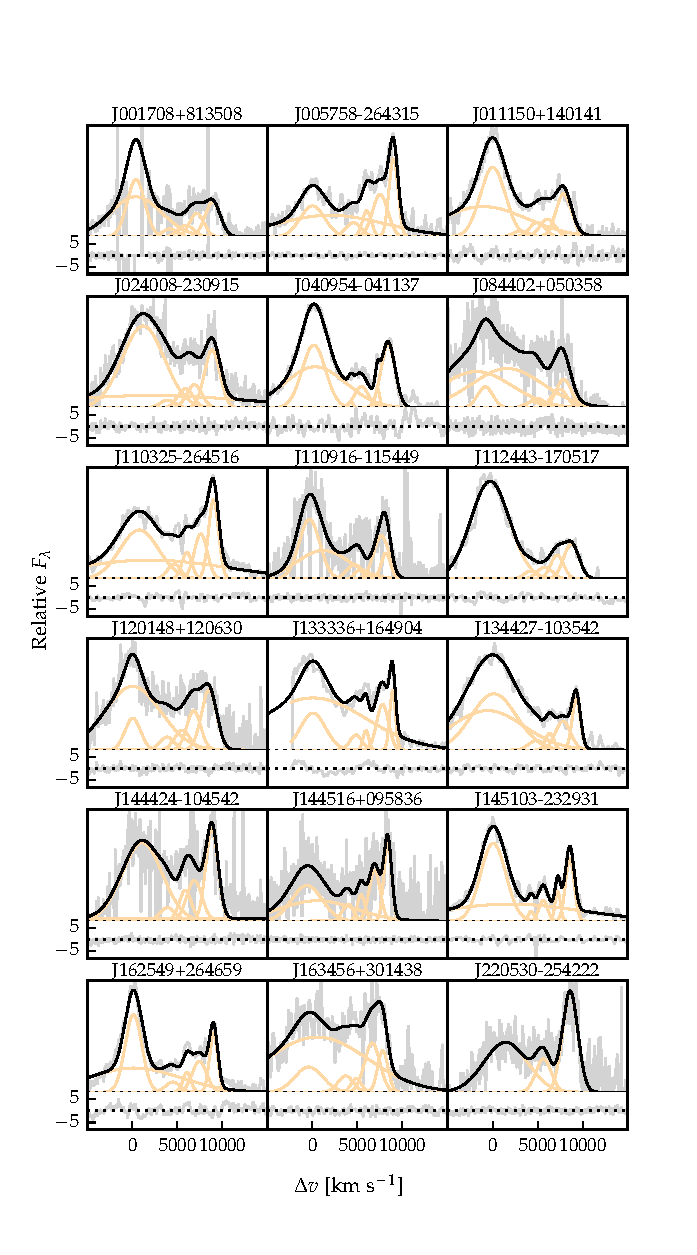
\includegraphics[width=1\columnwidth]{figures/chapter04/example_spectrum_grid_extreme_oiii.pdf} 
    \caption{Model fits to the continuum- and \ion{Fe}{II}-subtracted \hbns/[\ion{O}{III}] emission in 18 quasars with extreme [\ion{O}{III}] emission profiles. The data is shown in grey, the best-fitting model in black, and the individual model components in orange. The peak of the [\ion{O}{III}] emission is used to set the redshift, and $\Delta{v}$ is the velocity shift from the rest-frame transition wavelength of \hb. Below each spectrum we plot the data minus model residuals, scaled by the errors on the fluxes.}     
    \label{fig:example_spectrum_grid_extreme_oiii}
\end{figure}

Figure~\ref{fig:example_spectrum_grid_extreme_oiii} shows the spectra of 18 objects which we visually identified as having exceptionally broad [\ion{O}{III}] emission profiles. 
For all of these objects the [\ion{O}{III}] emission is heavily blended. 
One consequence of this is that there is a significant degeneracy when the emission is decomposed in to individual contributions from \ion{Fe}{II}, \hb and [\ion{O}{III}]. 
We note that there is a similarity between these objects and the four quasars presented in \citet{zakamska16}. 
\todo{Say more about this and compare to WIISH sample}

\subsubsection{Comparison}

In Figure~\ref{fig:redshift_comparison} we compare systemic redshift estimates made using [\ion{O}{III}], \hb and \ha. 
The scatter is around 300\kms. 
There is a small offset, such that [\ion{O}{III}] is normally slightly bluer than expected. 

\subsection{[\ion{O}{III}] and \ion{C}{IV} outflows are linked}


\begin{figure}
    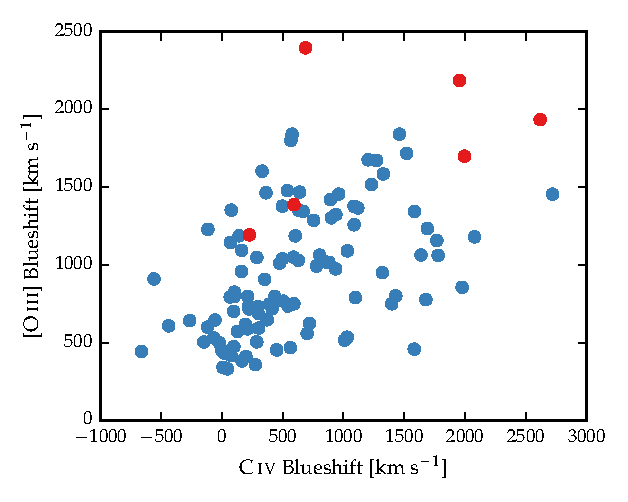
\includegraphics[width=\columnwidth]{figures/chapter04/civ_blueshift_oiii_blueshift.pdf} 
    \caption{The relation between the blueshifts of \ion{C}{IV} and [\ion{O}{III}].}     
    \label{fig:oiii_civ_blueshifts}
\end{figure}

Optical spectra are available for XXX quasars in our catalogue, and cover the broad \ion{C}{IV} doublet. 
As we described in Chapter~\ref{ch:bhmass}, \ion{C}{IV} is often blueshifted, which almost certainly signal the presence of strong outflows, most likely originating in a disc wind.
In Chapter~\ref{ch:bhmass} we demonstrated that the quasars in our sample cover the full range of \ion{C}{IV} blueshifts seen in the \ac{SDSS} quasar population, which makes our sample unique in that it allows us to study properties of the quasar across the full parameter range. 

The \ion{C}{IV} velocity centroid measurements are taken directly from Chapter~\ref{ch:bhmass}. 
We define the `location' of the [\ion{O}{III}] emission using $v_{10}$, although the results are the same if $v_{20}$ is used instead.
Note that we are using $v_{50}$ for the \ion{C}{IV} position. 
We can't use $v_{50}$ for [\ion{O}{III}] because sometimes we are using a single Gaussian, especially if the [\ion{O}{III}] is weaker and we miss the broad component.

In Figure~\ref{fig:oiii_civ_blueshifts} we show the \ion{C}{IV} blueshifts against the [\ion{O}{III}] blueshifts.
This comparison is done for a sub-sample of 146 objects where we have good measurements of the \ion{C}{IV}, [\ion{O}{III}] profiles. 
\todo{What is good?}

There is a clear and strong correlation. 
Note that our EQW cut removes most of the quasars with large \ion{C}{IV} blueshifts, since [\ion{O}{III}] is on average very weak in these quasars. 
Similar correlations have been tentatively found in lower redshift quasars and \ac{AGN} \citep{zamanov02}. 

The blueshifting of \ion{C}{IV} is known to correlate with luminosity \citep{richards11}.
In [\ion{O}{III}], the blueshifted wing becomes relatively more prominent as the luminosity of the quasar increases \citep{shen14}. 
Therefore, it is plausible that the correlation between the \ion{C}{IV} and [\ion{O}{III}] blueshifts is a secondary effect that is driven by the correlation of each with the luminosity. 
However, no strong luminosity-dependent trends are apparent in Figure~\ref{fig:oiii_civ_blueshifts}. 
We find that both the [\ion{O}{III}] and \ion{C}{IV} blueshifts are correlated with the luminosity, but that these correlations are much weaker than the correlation between the [\ion{O}{III}] and \ion{C}{IV} blueshifts. 


\todoinline{Also, you could put some more text and maybe a figure to explicitly demonstrate that the trend remains even after you have accounted for the trends with luminosity. This is the highlight result for me and personally I think needs a little more fleshing out.}

\section{Broad Absorption Line Quasars}

\todo{Check all of this}
19 quasars in our catalogue are classified as broad absorption line (BAL) quasars, using the either the \ac{SDSS} classification flags or the \citet{allen11} catalogue. 
We find that the BAL quasars have typically broader [\ion{O}{III}] than the rest of the sample. 
Note that in the \citet{zakamska16} sample of very red quasars, the incidence of BALs is very high, and these objects have extremely broad [\ion{O}{III}] profiles. 
A two-sided Kolmogorov-Smirnov statistic on the $w_{80}$ distributions returned a p-value of 0.10. 
What does this mean?
Try with different parameters?
Histograms look rubbish so maybe just give the numbers. 

\section{Discussion}

Looking at the [\ion{O}{III}] velocity width as a function of luminosity tells us about the physical drivers of the outflows observed in [\ion{O}{III}]. 
The correlation with luminosity suggests that the highest velocity outflows are associated with the most luminous \ac{AGN}. 
This has been reported for low-redshift \ac{AGN}, for both ionized and molecular outflows (e.g. Westmoquette et al. 2012; Veilleux et al. 2013; Arribas et al. 2014; Cicone et al. 2014; Hill \& Zakamska 2014).

This suggests that the outflows are driven by radiative forces. 
On the other hand, \citet{mullaney13} find that once the correlation between the [\ion{O}{III}] luminosity and the radio luminosity has been taken in to account, the [\ion{O}{III}] velocity width is more strongly related to the radio luminosity of the \ac{AGN}. 

Is the \ac{AGN} \ac{NLR} absent in objects where outflows have reached kilo-parsec scales, sweeping up the low-density material responsible for the [\ion{O}{III}]-emission?
If the \ac{BLR} outflows can escape, they are very fast and wouldn't need long to clear out the \ac{NLR} gas. 
\todo{Might be useful to estimate a time-scale for how long the NLR would take to be cleared given typical size of galaxy and velocity of outflow}. 

\subsection{Type II quasars}

Implications of our findings on searches for high-redshift type II quasars. 
It could be that type II quasars exist. 
If you look at CIV/MgII the narrow line components are very weak. 
So the contribution from the \ac{BLR} is very weak in luminous quasars, and you just won't see it even if the broad line region is obscured.
Findings in this paper seem to suggest that the static \ac{NLR} is very weak in luminous quasars. 

\todo{Wasn't too sure about what this section was trying to say... Have you considered the \ac{SDSS} Type 2 samples from e.g. Alexandroff et al. ? (http://adsabs.harvard.edu/abs/2013MNRAS.435.3306A). I thought those were pretty luminous, narrow-line objects?}

\section{ICA}

Then having presented the main results, I would go on to discuss the limitations of the Gaussian approach - e.g. FeII can't be properly subtracted in many cases and sensitive to S/N - and use this as an intro to the much more flexible ICA method. You could then have a much briefer description of the ICA reconstructions and present this more as work in progress. You could show that your main results (as above) still hold with the ICA (e.g. Figs 1.15, 1.16, 1.17) and that this allows you to solve the FeII problem and push to lower SNR. Finally, you could discuss some of the potential improvements to the ICA components that would allow the derived line properties from the ICA to become even more robust. ICA works better at low S/N because we are effectively putting priors on the model parameters. 


The second model consists of six spectral components derived from an \ac{ICA} of a large sample of low-redshift \ac{AGN} with \ac{SDSS} spectra covering the same spectral region.
As we will demonstrate, a linear combination of these spectral components is able to reproduce the spectra around \hbns/[\ion{O}{III}] to a high degree of precision.  

\subsection{Model Two: Independent Component Analysis}

\ac{ICA} is a blind source separation technique for separating a signal in to linearly mixed statistically independent subcomponents. 
Unlike the more widely-used principle component analysis technique, \ac{ICA} produces non-negative components which allows for a physical interpretation of the components and weights.  
\ac{ICA} has been succesfully applied to model the spectra of emission-line galaxies \citep{allen13} and BAL quasars \citep{allen11}. 
The quasar spectra can be thought of as a set of observations, $\bm{x}$, which are made up of statistically independent components, $\bm{c}$, that are combined by some mixing matrix, $\bm{W}$:

\begin{equation}
    \bm{x} = \bm{W}\bm{c}
\end{equation}

\ac{ICA} reverses this process and describes how the observed data are generated. 
Both the independent components and the mixing matrix are unknown, but can be found by solving:

\begin{equation}
    \bm{c} = \bm{W}^{-1}\bm{x}.
\end{equation}

The components were solved for using a sample of 2,154 \ac{SDSS} quasars at redshifts XX. 
\todo{Ask Paul for details.}
At these redshifts the \ac{SDSS} spectrograph covers the rest-frame region XX-XX\AA\, where \hb and [\ion{O}{III}] lie. 
The individual spectra were first adjusted to give the same overall shape as a model quasar template spectrum.
Six positive independent components and four additional components that could be negative were found to be sufficient to reconstruct the spectrum, without over-fitting. 
Each quasar spectrum $x_j$ can then be represented as a linear combination of the independent components: 

\begin{equation}
    x_j = \sum_{i=1}^{10} c_{ij}W_{ij}
\end{equation}

\subsubsection{Fitting procedure}

Each of the individual \ac{ICA} components has been adjusted to give the same overall shape as a quasar template spectrum. 
We approximate the overall shape of this template by fitting a single power-law to emission line free windows at 4200-4230, 4435-4700 and 5100-5535 \AA. 
We then flatten each of the \ac{ICA} components by dividing by this power-law. 
An identical process is performed on each spectrum we fit, so that both the components and the spectrum to be fitted have essentially zero shape. 
For each quasar in our sample we perform a variance-weighted least-squares minimisation to determine the optimum value of the components weights.
The first six component weights are constrained to be non-negative, and the fit is done in logarithmic wavelength space, so that each pixel corresponds to a fixed velocity width.   
The relative shift of the \ac{ICA} components is also allowed to vary in the optimisation procedure, to account for errors in the systemic redshifts used to transform the spectra in to rest-frame wavelengths. 

\subsubsection{Quality of fits}

In general, the \ac{ICA} components do a remarkably good job at reconstructing the spectra of the objects in our sample. 
\todo{Is there some way to demonstrate/quantify this?}
For example, in J125141+080718 (discussed above), it does much better job at modelling the \ion{Fe}{II} emission than the \citet{boroson92} template. 
It is less sensitive to the spectral \ac{S/N}, and the component weights do not need to be constrained. 
It is therefore much simpler to apply than fitting multiple Gaussians. 

However, it does have its limitations. 
The components were calculated using a set of lower-redshift, lower-luminosity \ac{AGN}, and quasar spectra are known to vary systematically as a function of luminosity. 
For example, the [\ion{O}{III}] line is typically broader in more luminous quasars. 
Because there are so few objects with very broad [\ion{O}{III}] in the low-redshift sample, the \ac{ICA} reconstruction fails to reproduce the broadest [\ion{O}{III}] profiles in our sample. 

\subsection{Physical interpretation of \ac{ICA} components}

\begin{figure}
    \centering
    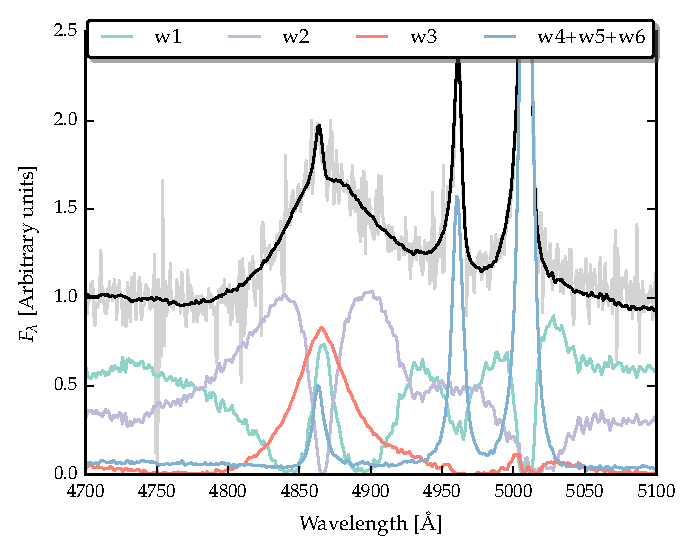
\includegraphics[width=0.8\textwidth]{figures/chapter04/mfica_components.pdf} 
    \caption{\hbns/[\ion{O}{III}] emission J002952+020607. The \ac{ICA} reconstruction is shown in black, and the spectrum in grey. The first three components, and the sum of components four, five and six are shown individually.}     
    \label{fig:mfica_components}
\end{figure}

Although the \ac{ICA} is analysis is not based on any physics,  there appears to be a direct correspondence between the individual components and the different emission features which contribute to the spectra (Fig.~\ref{fig:mfica_components}). 
This correspondence is summarised in Table~\ref{tab:icacomps}. 
The component $w_1$ seems to correspond to \ion{Fe}{II} emission, the components $w_2$ and $w_3$ to broad \hb emission, the components $w_4$ and $w_5$ to narrow [\ion{O}{III}] emission at the systemic redshift, and the component $w_6$ to broad, blueshifted [\ion{O}{III}] emission. 

\begin{table}
  \centering
  \small
  \caption{Physical interpretation of the \ac{ICA} components.}
  \label{tab:icacomps}
    \begin{tabular}{cc} 
    \hline
    Component & Origin \\
    \hline
    $w_1$& \ion{Fe}{II} \\
    $w_2$& \hbns \\
    $w_3$& \hbns \\
    $w_4$& [\ion{O}{III}] core \\
    $w_5$& [\ion{O}{III}] core \\
    $w_6$& [\ion{O}{III}] wing \\
    \hline
    \end{tabular}
\end{table} 

\subsubsection{Reconstructing the [\ion{O}{III}] profile}

\begin{figure}
    \centering
    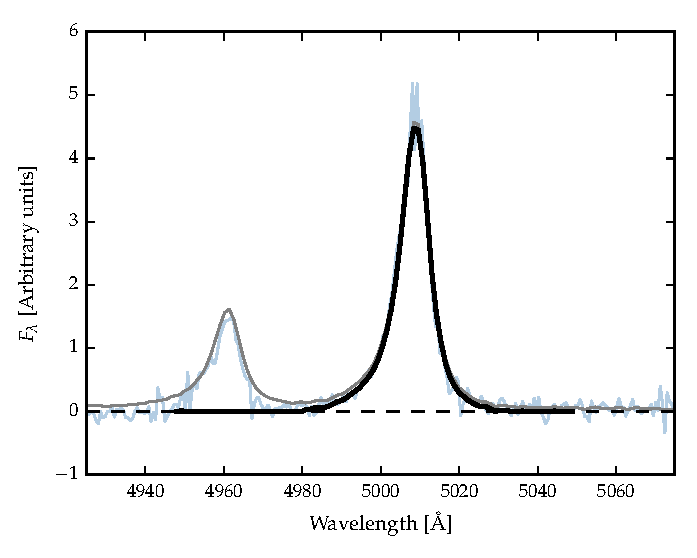
\includegraphics[width=0.8\textwidth]{figures/chapter04/oiii_reconstruction.pdf} 
    \caption{[\ion{O}{III}] emission in J002952+020607. The data is shown in blue, and the \ac{ICA} spectrum in grey. The first three \ac{ICA} components have been subtracted from both the \ac{ICA} composite and the data. The black curve shows the reconstructed [\ion{O}{III}] profile.}     
    \label{fig:oiii_reconstruction}
\end{figure}

In order to measure non-parametric line parameters, e.g. $v_{10}$, we must first reconstruct the [\ion{O}{III}] emission. 
It is fortunate that most of the [\ion{O}{III}] emission is in just three of the \ac{ICA} components; the remaining three contribute very little. 
Therefore, we can set the first three weights to zero to leave only the [\ion{O}{III}] emission. 
The four correction components are also included. 

We define the boundaries of [\ion{O}{III}]\l5008 as being between 4950 and 5500\AA. 
The blue limit is close to the peak of the [\ion{O}{III}]\l4960 line, and so to recover the intrinsic profile we instead use the blue wing of [\ion{O}{III}]\l4960. 
We use the emission from 4980-5050\AA, and from 4900-(4980-(5008.2-4960.3)). 
The blue window is then shifted by (5008.2-4960.3) to reconstruct the blue wing of the [\ion{O}{III}]\l5008 line. 
We then subtract a constant, because the flux does not always go to zero (suggests that there is probably flux which is not due to [\ion{O}{III}] emission in components four to six). 

An examples of a reconstructed [\ion{O}{III}] emission line is shown in Figure~\ref{fig:oiii_reconstruction}. 
\todoinline{At present I am summing the flux all the way from 4950\AA. However, this is quite a lot of flux to sum up, and we can't ascribe this flux to the wing of the [\ion{O}{III}] emission with any certainty. This is borne out by the fact that there are quite large differences between, for example, $v_{10}$ measured from the Gaussian fit and $v_{10}$ measured from the \ac{ICA} fit.} 

Unfortunately, there are systematic differences between the line-width estimates from the Gaussian reconstructions and the ICA reconstructions, particularly for broad-line objects.
The current way of doing the ICA reconstruction of the [\ion{O}{III}] line ignores any cross-talk between the components and there is potentially flux being ascribed to the line that could be coming from some other component. 
We can solve this by finding some more representative broad [\ion{O}{III}] lines in \ac{SDSS} from which to derive the components as well as producing a set of components for [\ion{O}{III}] only.
Therefore we don't use these reconstructions and leave this for future work. 

\subsection{\ac{ICA} fits}

\begin{figure}
    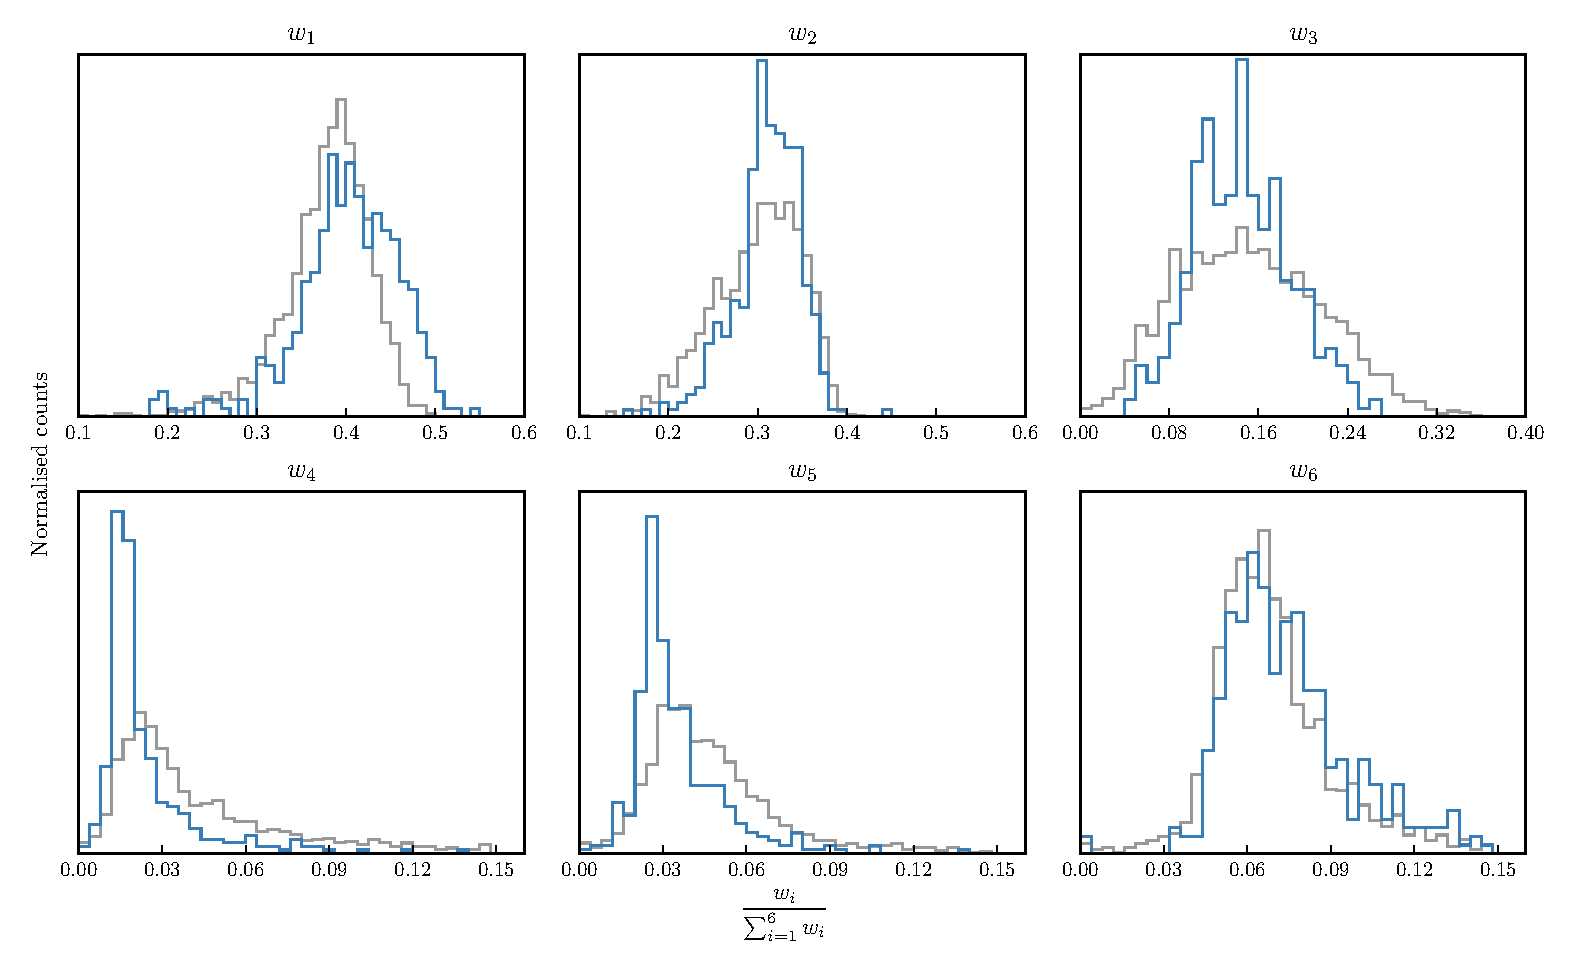
\includegraphics[width=\textwidth]{figures/chapter04/mfica_component_weights.pdf} 
    \caption{The relative weight in each of the six positive \ac{ICA} components for the high-luminosity (blue) and low luminosity samples (grey). In the high-luminosity sample \ion{Fe}{II} emission is stronger (component $w_1$). The core [\ion{O}{III}] emission (components $w_4$, $w_5$) is weaker but the strength of the blueshifted wing ($w_6$) is the same.}     
    \label{fig:mfica_component_weights}
\end{figure}

\begin{figure}
    \centering
    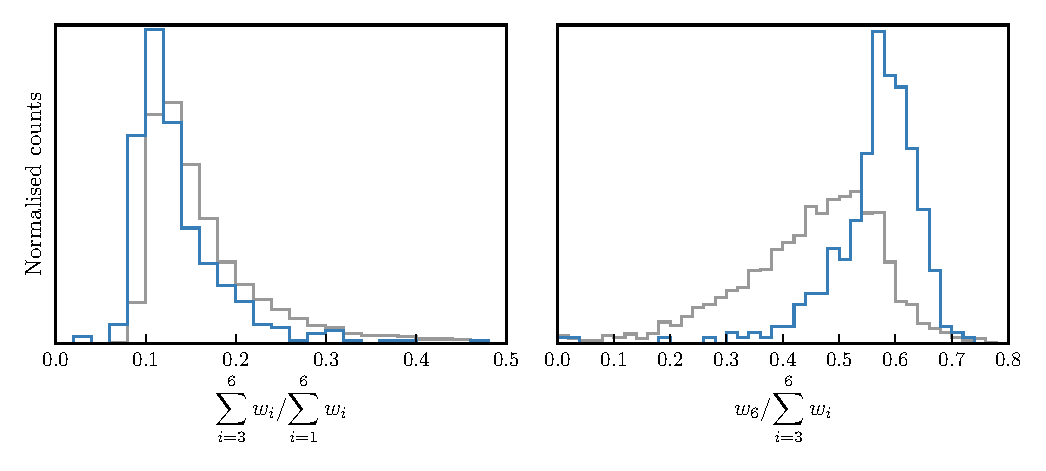
\includegraphics[width=\textwidth]{figures/chapter04/mfica_oiii_weight.pdf} 
    \caption{The relative weight in the three \ac{ICA} components corresponding to [\ion{O}{III}] emission ({\em left}) and the relative weight of the component most closely related to blueshifted [\ion{O}{III}] emission relative to all three [\ion{O}{III}] components ({\em right}). [\ion{O}{III}] emission is weaker in the high-luminosity sample, but the relative contribution from the blueshifted component to the total [\ion{O}{III}] emission is higher.}     
    \label{fig:mfica_oiii_weight}
\end{figure}

\begin{figure}
    \centering
    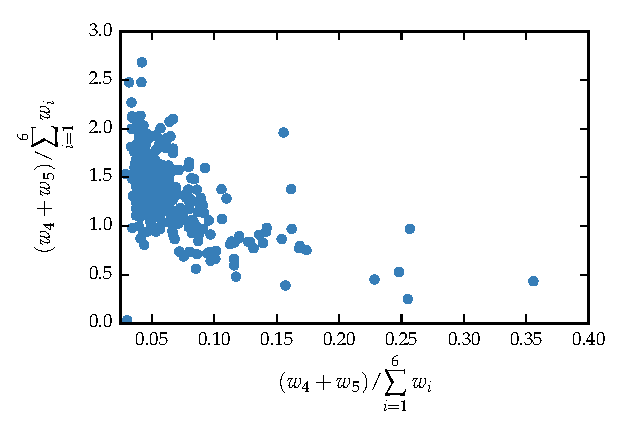
\includegraphics[width=\columnwidth]{figures/chapter04/oiii_core_strength_blueshift.pdf} 
    \caption{Weight in the [\ion{O}{III}] wing relative to the weight in the [\ion{O}{III}] core emission versus the strength of the core [\ion{O}{III}] emission. The blue-asymmetry of the [\ion{O}{III}] emission increases as the strength of the core component decreases.}     
    \label{fig:oiii_core_strength_blueshift}
\end{figure}

In Figure~\ref{fig:mfica_component_weights} we show the relative weights of each of the six positive \ac{ICA} components. 
Also shown are the same measurements for a sample of low-redshift, low-luminosity AGN. 
We want to examine whether or not there are systematic differences between these two samples. 

We see that [\ion{O}{III}] core emission is weaker in the more luminous sample, but the strength of the wing component is similar. 
\citet{shen14} showed that the strength of the core [\ion{O}{III}] component decreases with quasar luminosity and optical \ion{Fe}{II} strength faster than the wing component, leading to overall broader and more blueshifted profiles as luminosity and \ion{Fe}{II} strength (or \ion{C}{IV} blueshift) increases. 
\citet{shen14} suggested that a stable \ac{NLR} is being removed by the outflowing material. 
Similarly, \citet{zhang11} found that the more the peak of the [\ion{O}{III}] line is blueshifted, the more the core component decreases dramatically, while the blue wing changes much less. 
Therefore, there is an anti-correlation between the strength of the core component and the relative strength of the wing component (Figure~\ref{fig:oiii_core_strength_blueshift}). 

To show this phenomenon more clearly, we plot the relative [\ion{O}{III}] strength and the [\ion{O}{III}] wing/core ratio in the high/low luminosity samples (Figure~\ref{fig:oiii_core_strength_blueshift}). 
We see that [\ion{O}{III}] is weaker in the high luminosity sample, but that the wing component is much stronger relative to the core component. 
\todo{Similar to behaviour of \ion{C}{IV}? Would suggests that the mechanism producing the two correlations is the same}. 

\subsubsection{\ac{EV1} correlations}

\begin{figure}
    \centering
    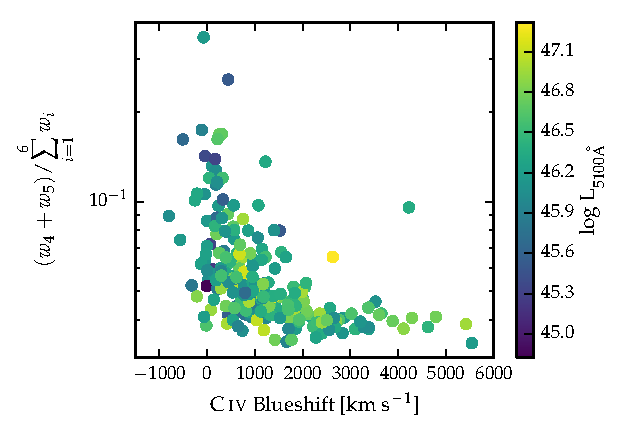
\includegraphics[width=\textwidth]{figures/chapter04/civ_blueshift_oiii_strength.pdf} 
    \caption{The \ac{ICA} component weight $w_4$, which is a proxy for the strength of core [\ion{O}{III}], as a function of the \ion{C}{IV} blueshift. The \ion{C}{IV} blueshift is measured relative to the NIR \ac{ICA} redshift.}     
    \label{fig:civ_blueshift_oiii_strength}
\end{figure}

\begin{figure}
    \centering
    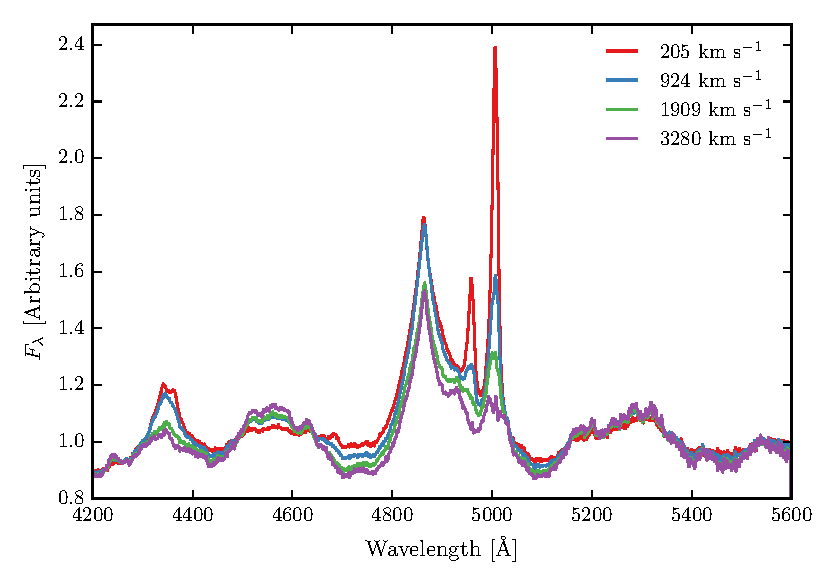
\includegraphics[width=\columnwidth]{figures/chapter04/mfica_composites.pdf} 
    \caption{Median \ac{ICA}-reconstructed spectra as a function of the \ion{C}{IV} blueshift.}     
    \label{fig:mfica_composites}
\end{figure}

In Figure~\ref{fig:civ_blueshift_oiii_strength} we show how the [\ion{O}{III}] strength varies as a function of the \ion{C}{IV} blueshift. 
There is a very well defined relation: when \ion{C}{IV} is strongly blueshifted [\ion{O}{III}] is very weak. 
This is very similar to what we found when we used Gaussian functions to model the emission. 
The correlation between \ion{C}{IV} blueshift and [\ion{O}{III}] EQW is shown in a different way in Figure~\ref{fig:mfica_composites}. 
Here we divide our sample in to four bins according to the \ion{C}{IV} blueshift. 
From the quasars in each \ion{C}{IV} blueshift bin we then find then generate an \ac{ICA} spectrum using the median weights from each quasar. 
The differences in the spectra as a function of the \ion{C}{IV} blueshift are dramatic. 
[\ion{O}{III}] becomes progressively weaker and more blueshifted.
The anti-correlation with \ion{Fe}{III} and the blue-ward \ion{Fe}{II} also clear, but there is no change in the redward \ion{Fe}{II}. 

\subsubsection{Updating \ac{EV1}}

The \ac{ICA} can be thought of as update on \ac{EV1}. 
The spectral diversity is encapsulated in the \ac{EV1} components. 
Most of the variance in \ac{EV1} is the anti-correlation between the strengths of [\ion{O}{III}] and \ion{Fe}{II}. 
So at one end we have objects with strong \ion{Fe}{II} and weak [\ion{O}{III}], and at the other end objects with weak \ion{Fe}{II} and strong [\ion{O}{III}]. 
Other properties, including the \ion{C}{IV} blueshift and the \hb \ac{FWHM}, also change systematically. 
Our work shows that the \ac{ICA} component weights change systematically along the \ac{EV1} sequence. 

\todo{Just present this as an idea for future work right at the end rather than having this sandwiched in the middle.} 
